
\section{Results}

\begin{frame}[c]{What does the deformation look like?}
	\begin{figure}[h]
		\centering
		\only<1>{
			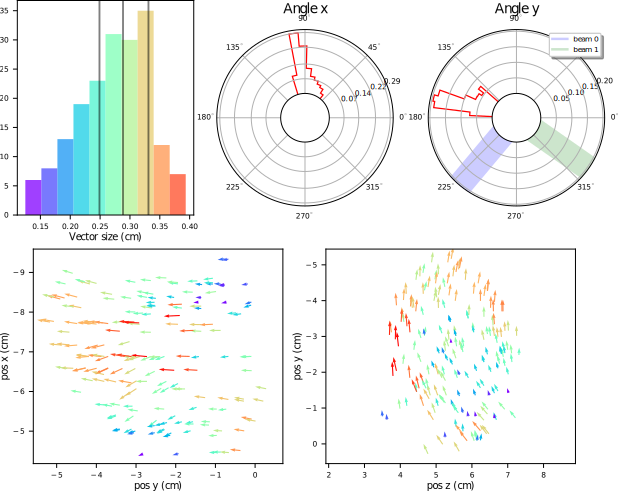
\includegraphics[height=0.8\textheight]{imgs/P015_cbct1_vf.pdf}
			\caption{Deformation field of patient 9, fraction 1}
		}
		\only<2>{
			\includegraphics[height=0.8\textheight]{imgs/P04_cbct1_vf.pdf}
			\caption{Deformation field of patient 4, fraction 1}
		}
	\end{figure}
	
\end{frame}

\begin{frame}[c]{How do the spot parameters change?}
	\centering
	\only<1>{
		\begin{figure}[h]
			\centering
			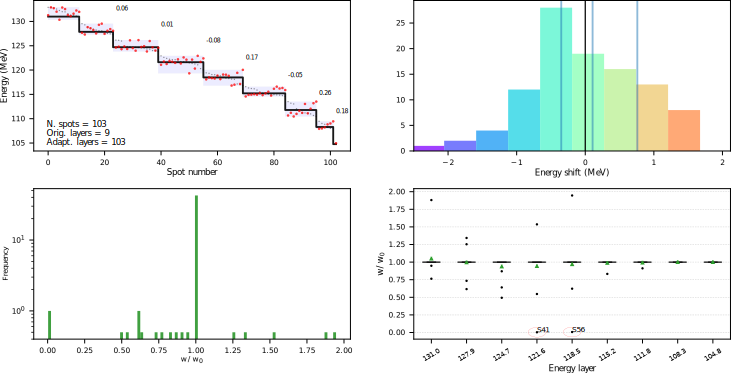
\includegraphics[width=\textwidth]{imgs/tramp_P02_cbct1.pdf}
			\caption{Fluence map changes: Patient 2, fraction 1, beam 1}
		\end{figure}
	}
	\only<2>{
		\begin{figure}[h]
			\centering
			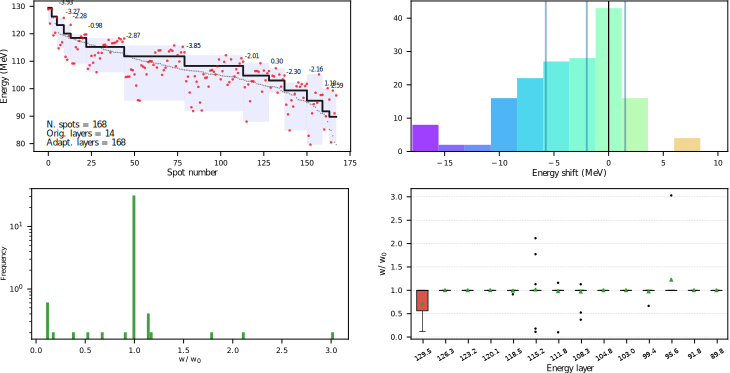
\includegraphics[width=\textwidth]{imgs/tramp_P10_cbct4.pdf}
			\caption{Fluence map changes: Patient 7, fraction 4, beam 2}
		\end{figure}
	}
\end{frame}


\begin{frame}[c]{Results: what has not worked}
	Geometric-only approaches:
	\begin{columns}[c]
		\begin{column}{0.55\textwidth}
			\begin{itemize}
				\item Not in the general case
				\item Divergences in the VF
				\item Bragg peaks changes
			\end{itemize}
		\end{column}
		\begin{column}{0.45\textwidth}
			\begin{itemize}
				\item Unbalance of spot doses
				\item Under-represented areas
				\item Constraints too strict
			\end{itemize}
		\end{column}
	\end{columns}
    \begin{figure}
        \only<2>{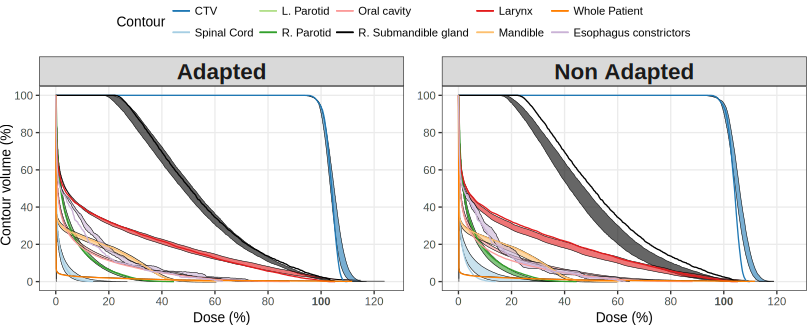
\includegraphics[width=\textwidth]{imgs/DVHs_normalized_Geo_free_P15_not_week6.pdf}}
        \onslide<3>{\includegraphics[width=0.9\textwidth]{imgs/target_V98_geometric_need_adapt.pdf}}
    \end{figure}
\end{frame}


\begin{frame}[c]{Results with weight tuning: CTV}
	Adjusting the weights shows improved results:
	\begin{figure}
        \includegraphics[width=\textwidth]{imgs/target_V98_weights_need_adapt.pdf}
    \end{figure}
    \onslide<2>{\textbf{Which one is better? Normalize and check homogeneity!!}}
\end{frame}


\begin{frame}[c]{Results with weight tuning: CTV}
    Normalized to V98 = 98\%:
    \begin{figure}
        \includegraphics[width=\textwidth]{imgs/target_D2_D98_weights_comparison.pdf}
    \end{figure}
    \ldots~hard to tell between \textit{Free} and \textit{Isocenter shift}. Maybe the OARs show a clearer pattern?
\end{frame}


\begin{frame}[c]{Results with weight tuning: OARs}
	The free strategy \textit{seems} slightly better than the isocenter strategy.
	\begin{figure}
		\only<1>{\includegraphics[width=\textwidth]{imgs/oars_mean_weights.pdf}}
		\only<2>{\includegraphics[width=\textwidth]{imgs/oars_max_weights.pdf}}
	\end{figure}
	The DVHs are normalized to V98 = 98\%.
\end{frame}


\begin{frame}[c]{Results overview}
    \only<1>{
    \begin{figure}[h]
        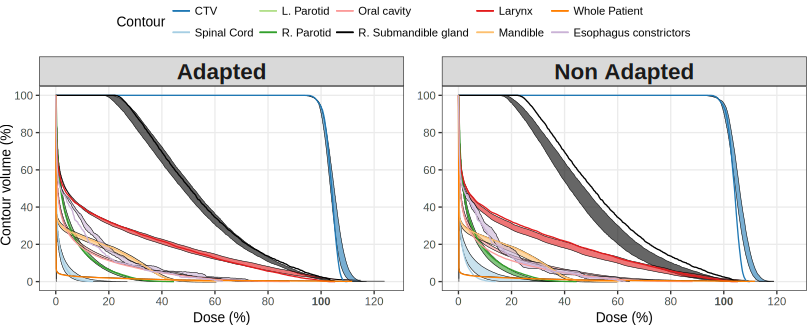
\includegraphics[width=\textwidth]{imgs/DVHs_normalized_Geo_free_P15_not_week6.pdf}
        \caption{Patient 9, adaptation vs plan}
    \end{figure}
    }
    \only<2>{
    \begin{figure}[h]
        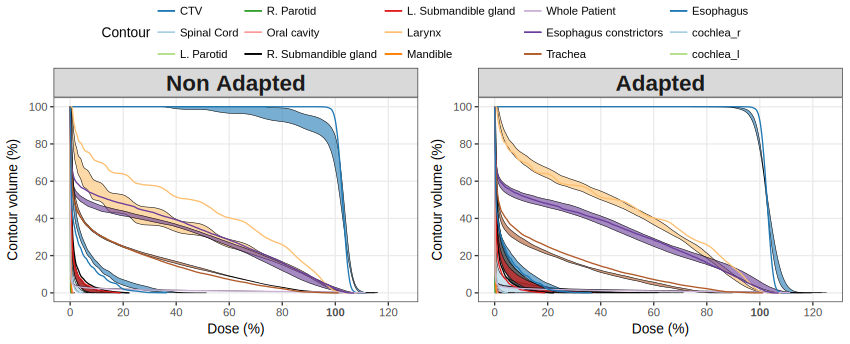
\includegraphics[width=\textwidth]{imgs/DVHs_Weight_Free_P10.pdf}
        \caption{Patient 7, adaptation vs plan}
    \end{figure}
    }
    \only<3>{
    \begin{figure}[h]
        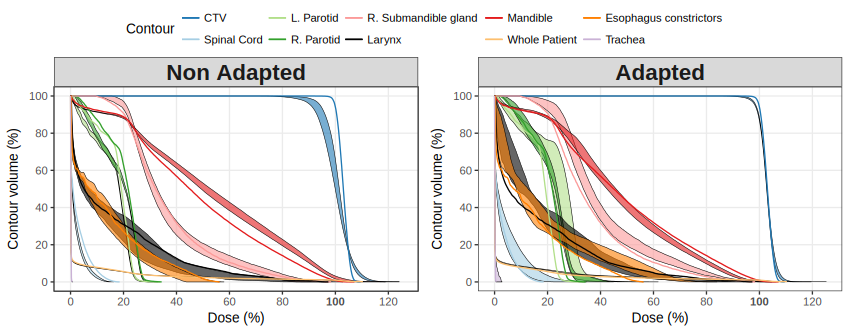
\includegraphics[width=\textwidth]{imgs/DVHs_Weight_Free_P14.pdf}
        \caption{Patient 8, adaptation vs plan}
    \end{figure}
    }
    \only<4>{
    \begin{figure}[h]
        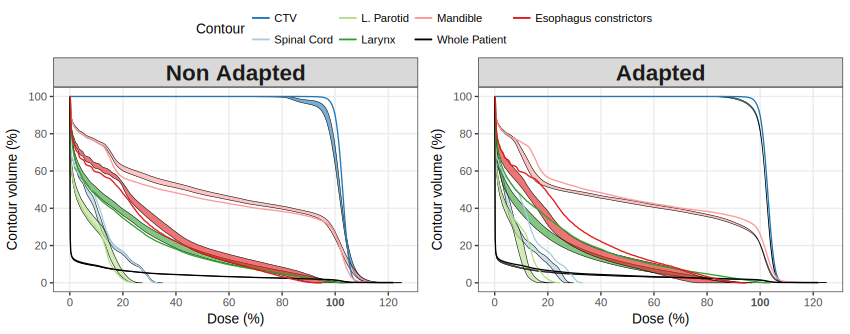
\includegraphics[width=\textwidth]{imgs/DVHs_Weight_Free_P07.pdf}
        \caption{Patient 6, adaptation vs plan}
    \end{figure}
    }
\end{frame}


\begin{frame}[c]{A quick peek into the next studies}
    \begin{figure}[h]
        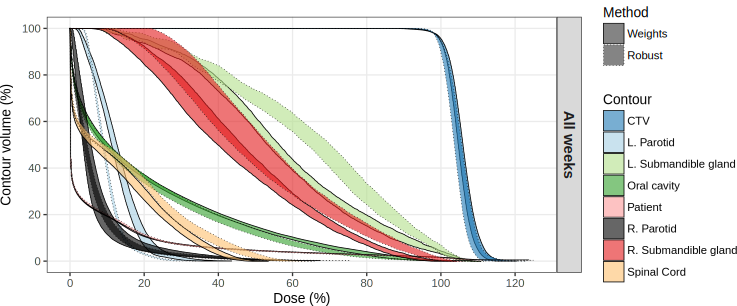
\includegraphics[width=\textwidth]{imgs/robust_opt.pdf}
        \caption{Patient 1, \textbf{adaptation vs ideal robust optimization}}
    \end{figure}
\end{frame}


\begin{frame}[c]{Timing, timing, timing!!}
    \begin{table}[h]
    \scalebox{0.8}{
        \begin{tabular}{l|ccc|c}
             & Minimum & Average & Maximum & Expected \\
            \hline
            Geometrical adapt. & 11.7  & 16.9  & 26.57 & $\sim1-5$ \\
            gPMC validation    & 115.6 & 261.9 & 419.2 & $\sim30$ \\
            Weight tuning      & 12.0  & 44.8  & 198.0 & ?? \\
            \hline
            Total              &   -   & 322.7 &   -   & $\sim60$ \\
            \hline
            $D_{ij}$ size (MB) & 4.1   & 77.9  & 312.0 & 50\% \\
            \hline
        \end{tabular}
        }
        \caption{Current and expected times}
    \end{table}
    Improvements:
    \begin{itemize}
        \item Geometrical adapt.: VF masks, binnings, multithreading\ldots
        \item gPMC validation: Multiple GPUs, unified codes, optimal stopping, kernel occupancy, thread variance reduction\ldots
        \item Opt4D optimization: I am not a great expert, but the dose matrices can be smaller
    \end{itemize}

\end{frame}
